Phase shift keying (PSK), faseskift modulering, brukes for å sende
digitale signaler.

En firkantpuls kommer inn på input, dette kombineres med en bærebølge.
Der hvor input skifter fra lav til høy, eller motsatt, får bærebølgen en
faseforskyvning på 180 grader.

\begin{figure}[H]
  \centering
  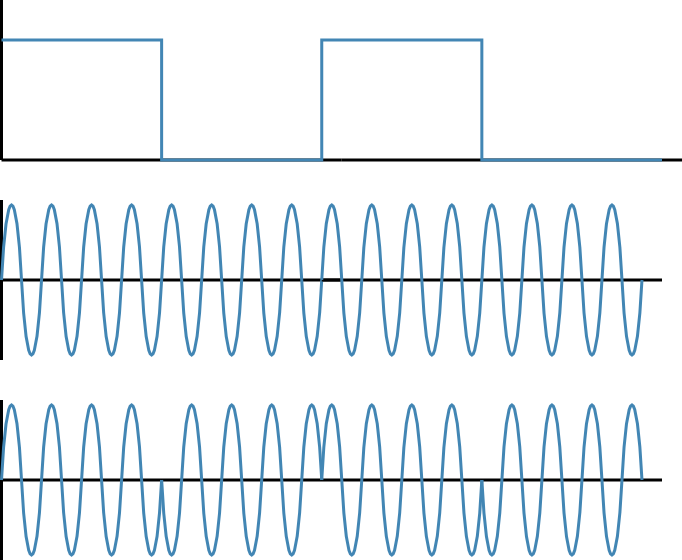
\includegraphics[width=0.67\textwidth]{./img/psk}
  \caption{Faseskift i overgang mellom lav/høy}
\end{figure}

Denne teknologien brukes i bl.a. WiFi, bluetooth og RFID.
